\documentclass[11pt, twocolumn]{article}
\usepackage{graphicx}
\author{Paul Batchelor}
\graphicspath{ {images/}}
\title{The Aesthetics of Project Orbit}
\begin{document}
\maketitle

\begin{abstract}

The goal of this paper is to outline design considerations for codename Project Orbit, an
isorhythmic sequencer for Ge Wang's Music 256a class at Stanford University. The outline
will be divided up into two sections. The first section will discuss design 
considerations found in relevant musical sequencers and interactive applications. The second
section will provide a detailed design proposal for Project Orbit.


\end{abstract}


\section{Relevant Design Aesthetics in Existing Software} 

\subsection{Applications to be Examined}
The following applications have been selected by the author as being aesthetically 
and musically relevant to his own sequencer that he is trying to create.


\paragraph{Bloom} is a generative music app by Brian Eno and Peter Chilvers. It is
the main source of inspiration for Project Orbit, due to its simple design and musical
brilliance.

Website: www.generativemusic.com

\paragraph{Osmos} is a physics-based game developed by Hemisphere Games. It has
been selected for its prominent use of the circle, and its satisfying audiovisual user experience.

Website: www.osmos-game.com


\paragraph{Poly} is a generative circle-based polyrhythmic sequencer app for 
iPad by James Milton. 

Website: http://james-milton.com/poly

\paragraph{Patterning} is a circular drum machine for the iPad by Olympia Noise co, 
that shows how circles can put a twist on a classic product.

Website: http://www.olympianoiseco.com/apps/patterning/

\subsection{Circular Sequencers}

Project Orbit at its very core is a \emph{circular sequencer}, where circles and
ellipses are used to display time. While not a novel concept, circular synthesizer 
are a captivating alternative 
to more "conventional" step sequencers, whose time is displayed in a more linear fashion. 

Circles are an intuitive representation of repeating phrases, and are ideal for visually displaying complex
rhythmic relationships.
\emph{Poly}, for instance, uses the circle as the 
basis for plotting complex polyrythms; the rate of a particular note element is
proportional to it's magnitude to the center of the screen. Circular sequencers have also be used to display Euclidean 
rhythms and isorhythms, the latter
of which is important to the design of Project Orbit.


\subsection{Isorhythms}

\emph{Isorhythms} are a technique used by composers to build polyrhythms and complex contrapuntal phrases.
Two or more repeating musical phrases of different durations are 
layered on top of one another. As time progresses, these phrases become more
and more out of phase with one another. Isorhythms often have a 
very hypnotic effect, and can be a way of utilizing grooves and looping without sounding repetitive. 

Brian Eno is noted as an artist and composer who heavily uses isorhythms in his ambient works.
\emph{"Music for Airports"}, for instance, uses isorhythms as the basis for many of the movements. 
More relevant to Project Orbit is his iPad app \emph{"Bloom"}, which can be viewed as a minimalist
isorhythmic sequencer. It is unsurprising that Eno has used isorhythms heavily in
his ambient music, as they effectively "smooth" out the implied meter of the composition. 

Isorhythms in Project Orbit will have single-note phrases repeating periodically in time. Size
of the period will be determined by its position relative to the center of the screen.

\subsection{Diegetic vs. Non-diegetic sound}

In film, diegetic and non-diegetic sounds can be roughly described as musical elements that 
are part of the environment on-screen (ex: a jukebox playing rock and roll in a diner), 
and sounds that are not created on-screen (ex: the Imperial March theme played when Darth Vader is on screen).
In the context of Project Orbit, diegetic/non-diegetic elements will refer to musical elements that 
the user can see and control and those that they cannot see or control.

In a sequencer, what happens when the user doesn't have 1:1 control of the sounds being created?
As more non-digetic elements are introduced, the application itself becomes more and more
of a realized composition and less of a sequencer. 
The author has a strong interest in blurring the line between composition and
traditional sequencing, and aims to incorporate that into Project Orbit. 
It can arguably be said that introducing a small amount non-diegetic elements into a
sequencer can heighten the immersion of the musical experience. 

The orchestration of \emph{Bloom} can be split up into two main sounds: the bell tones 
(diegetic), and the drones (non-diegetic). The drones are a generative background texture,
heavily influenced by the bell-like tones that the user makes. These drones are subordinate to 
the bells. They do not overwhelm or overpower, they are simply background accompaniment. 
Without the non-diegetic, the overall mix would sound very sparse.

\emph{Osmos} is another counter-example to \emph{Bloom}, where instead non-diegetic sounds
overpower the diegetic sounds. Despite this lack of control, Osmos still
proves to be a statisfying interactive sonic experience, as the diegetic sounds that can be created through
movement and absorption blend well with the non-diegetic atmospheric 
soundtrack.

Project Orbit aims to have a balance of diegetic/non-diegetic elements similar
to that of Bloom.


\subsection{Decay and Opacity}

Decay over time is an important design consideration for a generative sequencer like 
Project Orbit. In \emph{Bloom}, user-generated bell sounds, 
though repeating periodically, eventually fade out over time. This small detail
adds great depth to it's musicality. Isorhythmic phrases that would otherwise be 
static and quickly boring instead have a more interesting evolution over time. When
sounds decay, they create space for more note events, which can encourage the user
to interact longer with the music.

In \emph{Bloom}, decay is represented by opacity. As note elements decay in volume 
over time, the opacity becomes more and more translucent until it disappers entirely.
It is indeed a very intuitive visual representation of decay. 

\subsection{Ambient design}
Project Orbit intends to provide an ambient audio-visual experience. There are several specific design considerations for creating ambient. For work related to Project Orbit, 
these considerations will include:

\begin{description}
    \item[Masked Meter] \hfill \\
        A sense of tempo and pulse will be well defined, but the implied meter
will be blurred. 
    \item[Gentle pacing] \hfill \\
        Timing and pace are a crucial part of creating a relaxing environment. 
There should be no jerky movements or sudden changes in overall speed. 
    \item[Stillness] \hfill \\
        The environment should invoke a sense of stillness in the user. Audio and
visual cues should inspire one to slow down.
 
    \item[Flow] \hfill \\
        A certain "flow" must be created and maintained. Just as a circle has no 
jagged edges, the ambient environment should not do anything that could jar the
audience. There can be no wrong notes or sharp transitions. 

    \item[Big Spaces] \hfill \\
       Upon entering an ambient environment, one should immediately get the 
sensation that they are a tiny particle in a gigantic universe. 
\end{description}



\section{Project Orbit: a design proposal}


\begin{figure}[p]
\centering
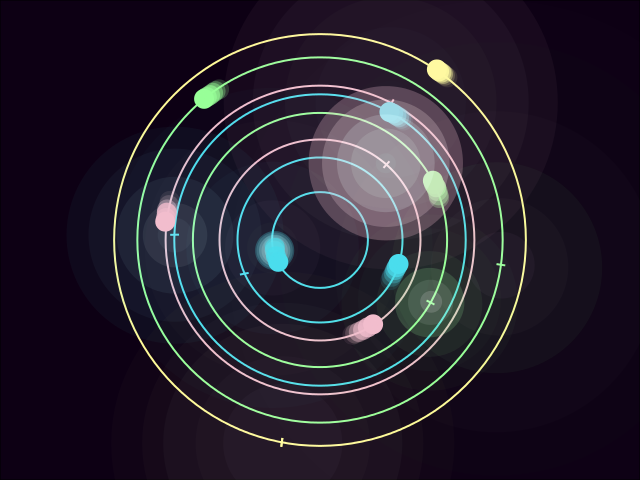
\includegraphics[width=\linewidth]{explosions}
\caption{Main design}
\label{fig:explosions}
\end{figure}

\begin{figure}[p]
\centering
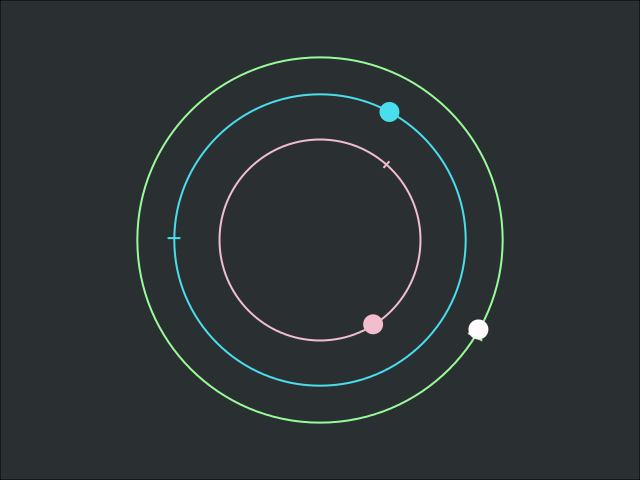
\includegraphics[width=\linewidth]{concept_sketch}
\caption{An earlier rendition of the main design.}
\label{fig:concept} \end{figure} 

\begin{figure}[p]
\centering
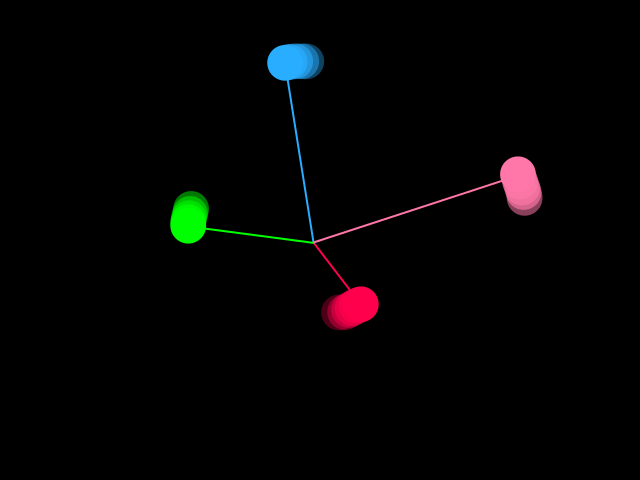
\includegraphics[width=\linewidth]{lines_and_circles}
\caption{Alternative design: A more minimal, "circles and lines" approach using 
the Pico8 color palette.}
\label{fig:lines_and_circles}
\end{figure}

\begin{figure}[p]
\centering
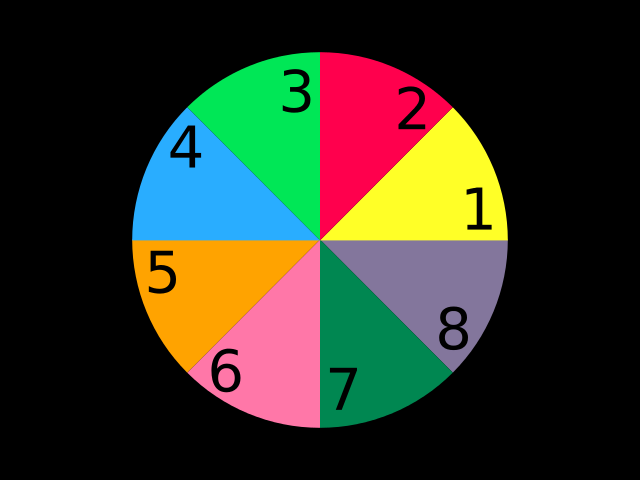
\includegraphics[width=\linewidth]{scale_positions}
\caption{Note values and voices are determined by where you click relative 
to the position in the unit circle. Timing is determined by the relative from the center
(the radius of the circle). }
\label{fig:scales} \end{figure} 

Project Orbit (temporary name) will be a 2-dimensional, isorhythmic, ambient sequencer, utilizing
the circle as the primary building block for design. When the program starts, a 
blank screen will be displayed. Clicking on the screen will draw a circle called a \emph{moon} that orbits
around the center screen. It's trajectory will be mapped by a circle, and it's origin will be defined by a 
small tick intersecting the circle.
Every time the moon the tick, it will produce
a note. The pitch and rotation time will be determined by X,Y position that the
user clicks on (See Figure ~\ref{fig:scales} for a breakdown of scales and positions.). 
After each rotation, the moons will decay, until they fade away. 


\subsection{Visual Considerations}
Visualizing the passage of time is important. For this reason, each moon will have
a ghost trail which will depict movement. 
It should be visually obvious when a moon 
has produced a note. The current proposed idea is to have the moon flash to white, and
to emit a ripple or shockwave. Figure ~\ref{fig:explosions} illustrates some of these visual considerations.

Visuals will be created using OpenGL primitives with use of color blending for 
opacity. Up for consideration will be the use of texture mapping to provide eye candy things like "glow". 
Shaders will be avoided for this particular project, as it exceeds
the authors limited knowlege of OpenGL. Some measures will taken for optimization in order
to make room for the sound engine.

The color palette for Project Orbit is currently in flux. 
Figure~\ref{fig:explosions} utilizes a pastel pallette, while
Figure~\ref{fig:scales} and Figure~\ref{fig:lines_and_circles} use the color pallette 
used in the Pico8 fantasy console system. 
%CITATION NEEDED HERE %

\subsection{Sound Considerations}

Stylistically, the music produced by Project Orbit will be generative ambient music. 
Flavors of
the pentatonic scale will be used, as these scales lend themselves well to generative
and interactive music. To fill in the empty spaces, non-diegetic sounds will be used. 

Initially, sound design for the instruments will consist of bell-like timbres and warm pads. 
Heavy amounts of reverb will be used to create a large space. All sounds will be
synthesized and not sampled. Techniques such as jitter, humanization, and layering will
be utilzed to add nuance to all the instruments and DSP.

For a sound engine, the author will utilize his own sound engines Soundpipe and Sporth 
to synthesize all the sound heard in Project Orbit. Sporth will provide a very
expressive syntax for composition. Soundpipe, whose abstraction is at a lower level 
than Sporth, will provide more efficient and fine tuned control of the sound synthesis.


\end{document}
